%%%%%%%%%%%%%%%%%%%%%%%%%%%%%%%%%%%%%%%%%%%%%%%%%%%%%%%%%%%%%%%%%%%%%%%%%%%%%%%%
%2345678901234567890123456789012345678901234567890123456789012345678901234567890
%        1         2         3         4         5         6         7         8

\documentclass[conference]{IEEEtran}
%\documentclass[letterpaper, 10 pt, conference]{ieeeconf}  % Comment this line out if you need a4paper

%\documentclass[a4paper, 10pt, conference]{ieeeconf}      % Use this line for a4 paper

\IEEEoverridecommandlockouts                              % This command is only needed if 
                                                          % you want to use the \thanks command

\overrideIEEEmargins                                      % Needed to meet printer requirements.

% See the \addtolength command later in the file to balance the column lengths
% on the last page of the document

% The following packages can be found on http:\\www.ctan.org
\usepackage{graphicx} % for pdf, bitmapped graphics files
%\usepackage{epsfig} % for postscript graphics files
%\usepackage{mathptmx} % assumes new font selection scheme installed
%\usepackage{times} % assumes new font selection scheme installed
\usepackage{amsmath} % assumes amsmath package installed
\usepackage{amssymb} % assumes amsmath package installed
%\usepackage[latin1]{inputenc}
\usepackage[brazilian]{babel}
\usepackage[utf8]{inputenc}
\usepackage[T1]{fontenc}
\usepackage[caption=false]{subfig}
\usepackage{url}
\usepackage{hyperref}

\addto{\captionsenglish}{\renewcommand{\abstract}{\bf \small \textit{Resumo---}}}

\title{\LARGE \bf
RoboIME: Team Description Paper}

\author{\IEEEauthorblockN{%
Carla~S.~Cosenza,
Clara L. de S. Santos,
Gustavo~C.~K.~Couto,
Jan~L.~L.~Segre,
Johnathan~F.~da~Rosa,\\
Luciano~de~S.~Barreira,
Luis~D.~P.~de~Farias,
Luis R. L. Rodrigues,
Matheus Bozza,\\
Onias~C.~B.~Silveira,
Renan~P.~de~Souza e
Paulo~F.~F.~Rosa}
\IEEEauthorblockA{%
\\Instituto Militar de Engenharia - IME
}
Rio de Janeiro - RJ\\
\url{www.roboime.com.br}
}

\begin{document}


\maketitle
\thispagestyle{empty}
\pagestyle{empty}


\begin{abstract}
This paper describes the electronic, mechanical and software designs developed by RoboIME Team in order to join LARC 2016. All designs are in agreement with the rules of Small Size League 2016. This is the fourth time RoboIME participates in the Latin American Robotics Competitions.

\end{abstract}


\section{Introdução}
A RoboIME é uma equipe de futebol de robôs da categoria Small-Size do Instituto Militar de Engenharia, Rio de Janeiro, Brasil. Esta é a sétima vez que o time participa de competições, sendo os maiores resultados um segundo lugar na RoboCup Brazil Open 2011 e um segundo lugar na LARC 2012. 

Todos os alunos que trabalham no projeto são membros do Laboratório de Robótica e Inteligência Computacional do IME. Estudos prévios \cite{tdp2014}\cite{tdp2012} serviram de referência para as atuais estruturas de \textit{software} e \textit{hardware} da equipe. Este artigo descreve os design computacionais, eletrônicos e mecânicos.

Este artigo está organizado da seguinte forma. Na seção 2, está descrito a nossa inteligência. O projeto eletrônico está descrito na seção 3. O \textit{design} mecânico é apresentado na seção 4. Finalmente, as conclusões e discussões sobre trabalhos futuros estão descritas na seção 5.

\section{SOFTWARE}
O \textit{software} da equipe RoboIME se baseia em 4 projetos: Core, Intel, SSL-Vision e grSim.

\subsection{Core}

O núcleo de processamento, o Core, é responsável por tratar as informações recebidas, atualizar a inteligência artificial (IA) com o estado do jogo e transmitir os comandos desta IA para os robôs.

O Core é composto por quatro módulos: Vision, Game State, Intel I/O e Simulação:

\subsubsection{Vision}

O componente de visão é responsável por receber os dados da SSL-Vision, unir os dados das 4 câmeras e aplicar filtros. Inicialmente será usado um filtro de passa baixa, mas também está sendo feito um esforço para modelar a física do jogo de forma a testar um filtro de Kalman, capaz não só de fazer a fusão dos dados das várias câmeras e estabilizar a posição dos robôs e da bola como também prever o estado futuro do jogo.

\subsubsection{Game State}

O Game State é responsável por armazenar o estado do jogo (posição e orientação dos robôs, posição da bola e estimativa da velocidade de cada objeto), o estado do juiz e os pacotes de comando (velocidade normal e tangencial, o estado do driblador e o chute de cada robô). O Game State é compartilhado com a Vision, Intel I/O e Control.

\subsubsection{Intel I/O}

É responsável tanto por iniciar o(s) processo(s) de inteligência artificial quanto por comunicar-se com estes. A comunicação é estabelecida - por meio de I/O padrão - entre o Core e um software (executável) capaz de realizar algoritmos de inteligência artificial que definirão a estratégia da equipe, basta que tal software corresponda ao protocolo de envio e de recebimento de dados definido. Tal arquitetura permite desenvolver um projeto de inteligência artificial portável, independente e indiscriminante quanto à(s) linguagem(ns) de programação utilizada(s).

\subsubsection{Simulação}

Consta de um simulador, ainda em desenvolvimento, interno ao Core. Este módulo não só simula a física envolvida em uma partida como também o juiz do jogo. Desta forma, os jogos podem ser executados de maneira automática e verossímil sem a necessidade de interferência nos jogos. De forma a tornar os testes mais dinâmicos e possibilitar o treino de algoritmos de aprendizagem.
Está sendo incluido no simulador tanto os modelos físicos da bola, como dos robôs e da câmera de forma a se aproximar o máximo possível da situação real de jogo.

 \subsection{Inteligência}
A inteligência computacional é o foco do projeto Intel. Com a posição e orientação que um robô pode ocupar em campo representada por uma pose $p = [x$\hspace{0.25cm}$y$\hspace{0.25cm}$\theta]^T$, uma trajetória viável e contínua que ligue duas poses representada por $P = \{ p_1, p_2, ..., p_n \}$, um robô representado por $r = [pose$\hspace{0.25cm}$raio]^T$, a bola representada por $b = [x$\hspace{0.25cm}$y$\hspace{0.25cm}$raio]^T$ e um estado de jogo representado por $E = \{R_o, R_a, b\}$ onde $R_o$ é o conjunto de robôs do nosso time e $R_a$ é o conjunto de robôs do time adversário. A primeira etapa do software de inteligência é responsável por analisar o atual estado de jogo $E_a$ e definir uma pose de interesse para um robô $r_o \in R_o$ caso exista a necessidade. O algoritmo de inteligência artificial  utilizado para o cálculo de poses de interesse ainda está sendo desenvolvido. Estuda-se a possibilidade de desenvolvimento de uma inteligência artificial baseada na arquitetura STP (\textit{Skill, Tactic, Play})\cite{stp}, no princípio de agentes autônomos ou em métodos heurísticos. Assim é definindo um estado de jogo futuro de interesse $E_f$ que precisa ser atingindo em um determinado período de tempo $t$. Na figura \ref{img:pose} encontra-se um exemplo de poses.
\begin{figure}[thpb]
	\centering
	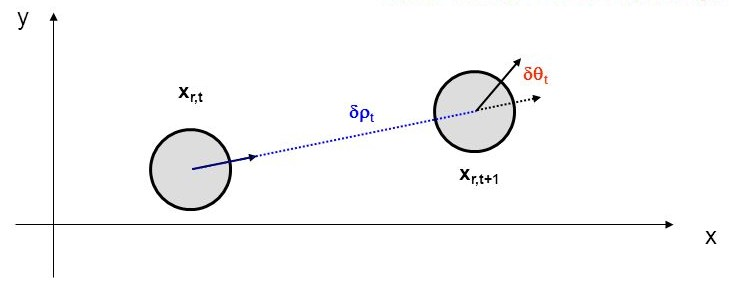
\includegraphics[width=\linewidth]{img/pose}
	\caption{Exemplo de poses que um robô pode assumir.}
	\label{img:pose}
\end{figure}

A segunda etapa do software de inteligência é responsável por verificar se uma nova pose de interesse $p_i$ foi definida para um robô $r_o$, caso sim, é executado um novo calculo da trajetória que ligará a pose atual $p_a$ do robô com a pose de interesse $p_i$. O calculo de trajetória é executado com auxílio da biblioteca OMPL (\textit{Open Motion Planning Library}) (Sucan et al, 2012)\cite{ompl} que implementa um apanhado de algoritmos de planejamento de trajetória, além de possibilitar otimizações quanto a suavidade do caminho gerado e o custo de movimento de uma pose atual para uma pose de interesse.

A terceira etapa do software de inteligência é feita em tempo de execução onde é utilizado a técnica campos potenciais (Goodrich, 2002)\cite{goodrich} para guiar os robôs de maneira reativa evitando colisões desenecessárias e seguindo suas trajetórias definidas na etapa anterior.

\section{Eletrônica}
%Eletrônica
A fim de produzir uma geração nova de robôs, a quarta na história do time, o projeto eletrônico está sendo reformulado esse ano com base no projeto antigo, mas com pequenas alterações visando aumentar tornar o projeto mais organizado e otimizar o processo de produção. Com isso o desenho das placas está sendo refeito do zero utilizando uma ferramenta de projeto nova para o time o \textit{Altium Designer}, sendo dada mais atenção ao dimensionamento das trilhas, escolha e posicionamento dos componentes.

A eletrônica dos robôs é baseada em uma arquitetura modular com foco em facilitar a rápida manutenção dos robôs em caso de falhas, manter baixo o custo de manutenção e tornar o projeto mais didático. O projeto eletrônico é dividido em 9 placas, uma placa mãe, 5 módulos de motor, um módulo de chute, um módulo de transmissão comercial (NRF24L01), um módulo de controle comercial (a stm32-discovery) e a placa mãe do robô.


Aproveitando as mudanças, o \textit{firmware} do robô também está sendo reescrito para ser implementando o conceito de abstração de \textit{hardware} e aumentando o caráter modular do projeto. Com esse objetivos em mente, o código está sendo mudado de C para C++, e foi dividido em classes que representam recursos físicos do microcontrolador e \textit{chips} do robô. A figura \ref{img:diagrama} ilustra o diagrama do funcionamento da arquitetura com abstração em \textit{hardware}, objetivo final do trabalho no firmware. Também está se passando a utilizar um sistema operacional de modo a possibilitar o uso de \textit{threads}.


\begin{figure}[thpb]	
	\centering
	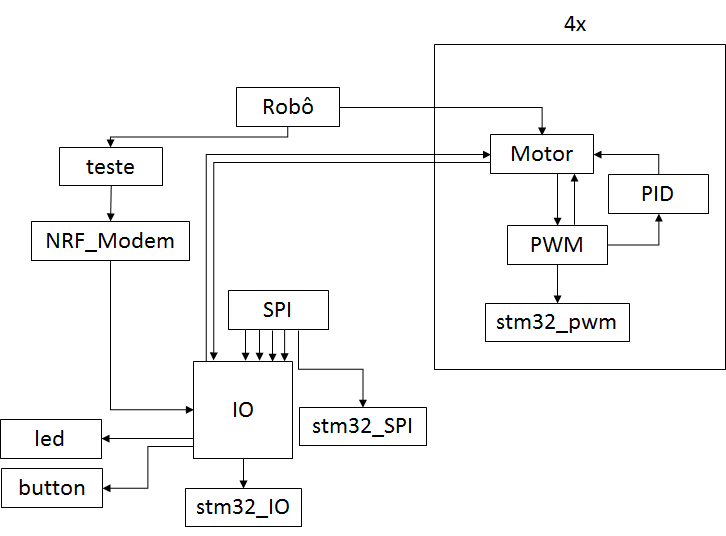
\includegraphics[width=\linewidth]{img/fluxograma_controle}
	\caption{Diagrama da arquitetura do \textit{firmware}.}
	\label{img:diagrama}
\end{figure}

\subsection{Módulo de controle}

O módulo de controle utilizado é uma placa STM32F4-Discovery (mostrada na figura \ref{img:modulocontrole}), comercializada pela \textit{STMicroelectronics}, contendo o microcontrolador STM32F407VG (de arquitetura ARM32 Cortex M4), responsável por realizar as operações lógicas do robô, servindo como cérebro do sistema eletrônico.


\begin{figure}[thpb]	
	\centering
	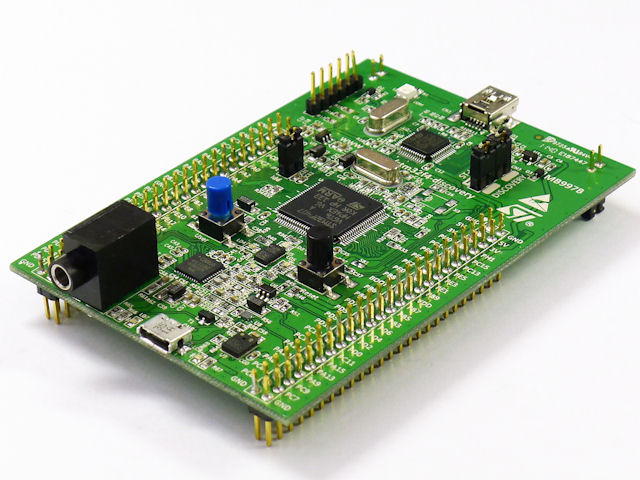
\includegraphics[width=\linewidth]{img/modulocontrole}
	\caption{Módulo de controle utilizado, placa STM32F4-Discovery. Fonte: \cite{omni}}
	\label{img:modulocontrole}
\end{figure}

Está sendo implementado esse ano um sistema operacional no módulo de controle. Segundo (Maziero,2013)\cite{maziero}, os objetivos básicos de um sistema operacional podem ser sintetizados em abstração de \textit{hardware} e gerência de recursos (quando dois ou mais aplicativos precisam dos mesmos recursos e cabe ao sistema operacional definir políticas para gerenciar o uso dos recursos de \textit{hardware} pelos aplicativos e resolver eventuais disputas).

Um sistema operacional dá a ilusão de que há várias tarefas sendo executadas a cada momento fazendo com que o processador alterne rapidamente de tarefa e delegando a cada tarefa uma fração do tempo de uso de processador adequada para sua execução. Isso é feito pelo agendador de tarefas (\textit{scheduler}).

O \textit{scheduler} e o controle omnidirecional das velocidades dos motores descritos a seguir são inovações para a equipe, sendo, portanto, a primeira competição em que serão usadas tais ferramentas.

\subsubsection{Uso de RTOS (\textit{Real Time Operating System})}

O \textit{scheduler} em um RTOS é feito para ter um padrão de execução previsível (determinístico). Isso é particularmente interessante para sistemas embarcados, pois é necessário que o sistema responda a um evento dentro de um intervalo de tempo bem definido (chamado de \textit{deadline}). \textit{Schedulers} de tempo real tradicionais, tais como o usado no \textit{FreeRTOS}, obtém determinismo permitindo ao usuário atribuir uma prioridade a cada linha de execução (\textit{thread}). O \textit{scheduler} usa a prioridade para saber qual a próxima \textit{thread} executar.

Por fim, \textit{FreeRTOS} é um RTOS gratuito, bastante popular, desenvolvido pela \textit{Real Time Engineers Ltd.} para ser pequeno o bastante para ser usado em microcontroladores. \textit{FreeRTOS} é distribuído sob a GPL (\textit{GNU Public License}) com uma restrição adicional e uma exceção opcional que permite que o código do proprietário seja fechado, mantendo apenas o \textit{kernel} código aberto.

Portanto, trata-se de um sistema operacional que permitirá a execução “simultânea” de tarefas de controle dos motores e comunicação do robô com a inteligência, atribuindo a cada tarefa uma fração de tempo determinada, sem aumentar muito o consumo de memória e usando um \textit{software} gratuito e amplamente difundido.

\subsubsection{Controle das velocidades}

Para  controle das velocidades, rodas omnidirecionais são usadas nos robôs. Embora potência seja perdida, já que cada motor atua apenas com uma componente de sua velocidade, o ganho por ter liberdade de movimento em todas as direções é substancial, pois diminui o número de ações que o robô terá de executar para se movimentar, ou seja, tornando-o mais ágil.

Para determinar as velocidades em cada motor sabendo as velocidades radial, tangencial e angular, uma matriz de transformação $D$ $(1)$ é utilizada. Na figura \ref{img:omni} temos o robô visto de cima, com os ângulos da matriz $D$. Multiplicando-a pela esquerda o vetor $v = [V_x$\hspace{0.25cm}$V_y$\hspace{0.25cm}$\omega r]^T$ temos o vetor $m = [V_1$\hspace{0.25cm}$V_2$\hspace{0.25cm}$V_3$\hspace{0.25cm}$V_4]^T$, que diz as velocidades que cada motor deve gerar.

% bizus para editar eqs latex:
% - https://www.codecogs.com/latex/eqneditor.php
% - http://www.hostmath.com/

\begin{equation}
    D = \begin{bmatrix}
        -\sin\varphi & \cos\varphi & 1 \\
        -\sin\varphi & -\cos\varphi & 1 \\
        \sin\theta & -\cos\theta & 1\\
        \sin\theta & \cos\theta &1
    \end{bmatrix}
\end{equation}

\begin{figure}[thpb]	
	\centering
	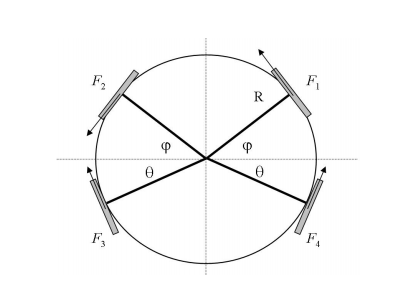
\includegraphics[width=\linewidth]{img/omni}
	\caption{Robô visto de cima. Fonte: \cite{omni}}
	\label{img:omni}
\end{figure}

Outra ferramenta interessante de usarmos essas rodas é verificar de forma simples se alguma roda está deslizando em uma camada acima do controle PID (Proporcional-Integral-Derivativo)(Ogata, 2003)\cite{ogata-pid}. Para isso, calcula-se a pseudo-inversa de $D$, $D^+$, e verifica-se se ($I-D\cdot D^+)\cdot m$ = 0. Se for diferente de zero, quer dizer que há deslizamento. Para corrigir isto, pega-se a primeira linha da matriz $I-D\cdot D^+$, gerando o vetor $u^T$. Então, o $m_c$ corrigido será dado pela retirada da projeção de $m$ em $u$. Algebricamente, $m_c = m - u\displaystyle\frac{<m,u>}{<u,u>}$. Desfeito o deslizamento, pode-se então proceder com o controle PID (Rojas, 2005)\cite{omni}.

\subsection{Módulo do motor}

Os módulos de motor (vistos na figura \ref{img:modulomotor}) fazem o controle dos quatro motores responsáveis pelo movimento do robô e do motor responsável pela atuação do driblador. Consiste em uma ponte H capaz de controlar a velocidade de um motor de corrente contínua em duas direções. 

\begin{figure}[thpb]	
	\centering
	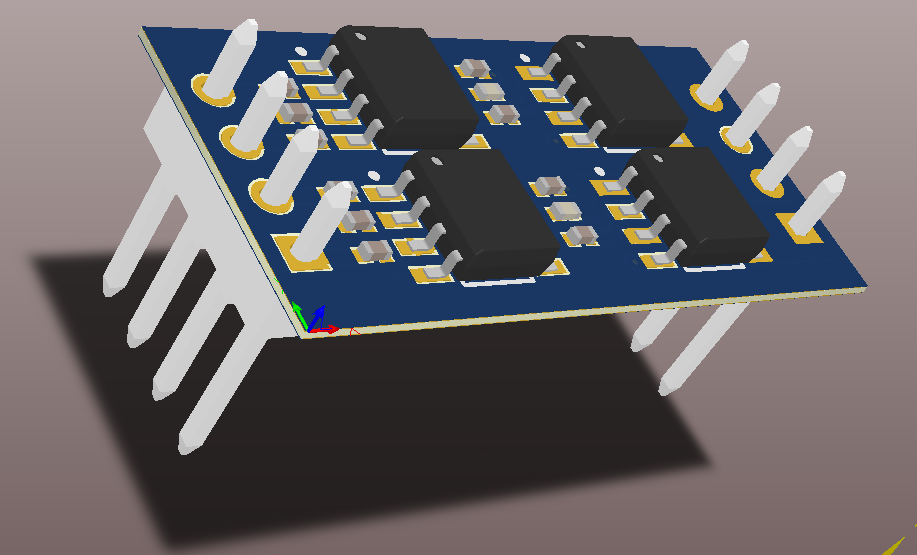
\includegraphics[width=\linewidth]{img/modulomotor}
	\caption{Módulo do motor.}
	\label{img:modulomotor}
\end{figure}

A placa é controlada pelo microcontrolador através da classe motor que utiliza a classe \textit{encoder} para determinar a velocidade instantânea do motor. Com essa velocidade utiliza-se um algoritmo de controle PID para calcular a resposta que deve ser transmitida a placa, e envia-se essa resposta utilizando as classes degrau unitário e PWM (\textit{pulse width modulation}).

O circuito de ponte H permite que o microcontrolador controle o sentido de rotação dos motores e a potência transmitida a eles, através do chaveamento dos transistores internos da ponte e amplificando o sinal enviado pelo microcontrolador.

O desenho dessa placa foi reformulado esse ano, as trilhas foram trocadas por planos nos caminhos de potência e foram adicionados um par de capacitores de desacoplamento na entrada dos \textit{drivers} dos transistores.

\subsection{Placa mãe}

A placa mãe (figura \ref{img:moduloplacamae}) é responsável por fazer a ligação entre os atores do robô, transmitindo potência da bateria para os módulos de motor e de chute, fazendo a ligação entre esses módulos e os respectivos atuadores, fornecendo tensão aos circuitos lógicos e fazendo a ligação entre o módulo de controle e os sensores do robô -, no caso um sensor de quadratura em cada motor e o sensor ótico do chute que verifica a posse da bola. 

\begin{figure}[thpb]	
	\centering
	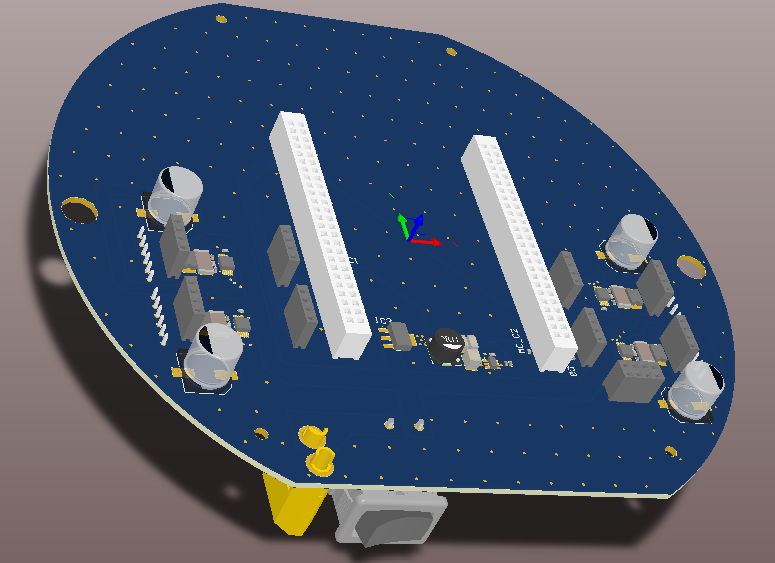
\includegraphics[width=\linewidth]{img/moduloplacamae}
	\caption{Módulo da placa mãe}
	\label{img:moduloplacamae}
\end{figure}

Para que as ligações feitas pela placa sejam feito de modo estável e seguro a placa mãe contém um fusível, um capacitor de tanque, um capacitor de desacoplamento, e um sensor de corrente, o \textit{chip} INA220, na entrada de cada módulo de motor e na entrada do módulo de chute, além de um circuito de divisão de tensão para que o módulo de controle seja capaz de controlar o nível de tensão da bateria.

O controle dessa placa é feito através da classe INA220 no \textit{firmware}, que faz a comunicação com os sensores de corrente na placa e a classe bateria que controla o nível da bateria sendo usada pelo robô. Essas classes permitem o controle dos circuitos de segurança do robô de maneira que o \textit{firmware} possa lidar com comportamento anômalos.

O desenho dessa placa foi reformulado esse ano, as trilhas nos caminhos de potência foram trocados por planos, os antigos fusíveis simples foram trocados por fusíveis resetáveis para evitar a troca em cada caso de comportamento anômalo. E os capacitores de tanque \textit{through hole} foram trocados por capacitores SMD (\textit{Surface-Mount Device}) visando automatizar o processo de montagem utilizando uma \textit{pick and place} automática.

Os sensores de corrente também foram trocados por sua versão mais moderna e foi corrigido um erro em sua implementação no esquemático. Outra pequena mudança foi a troca do conector do módulo de transmissão para ser compatível com o novo módulo de transmissão adotado pelo time.

\subsection{Módulo de chute}

O mecanismo de chute do robô foi elaborado utilizando dois solenoides como atuadores, um responsável pelo chute para frente e outro responsável pelo chute alto. E a placa (vista na figura \ref{img:modulochute}) é responsável por produzir a alta tensão necessária para ativar os dois solenoides, e transmitir a energia acumulada para acionar os atuadores.

\begin{figure}[thpb]	
	\centering
	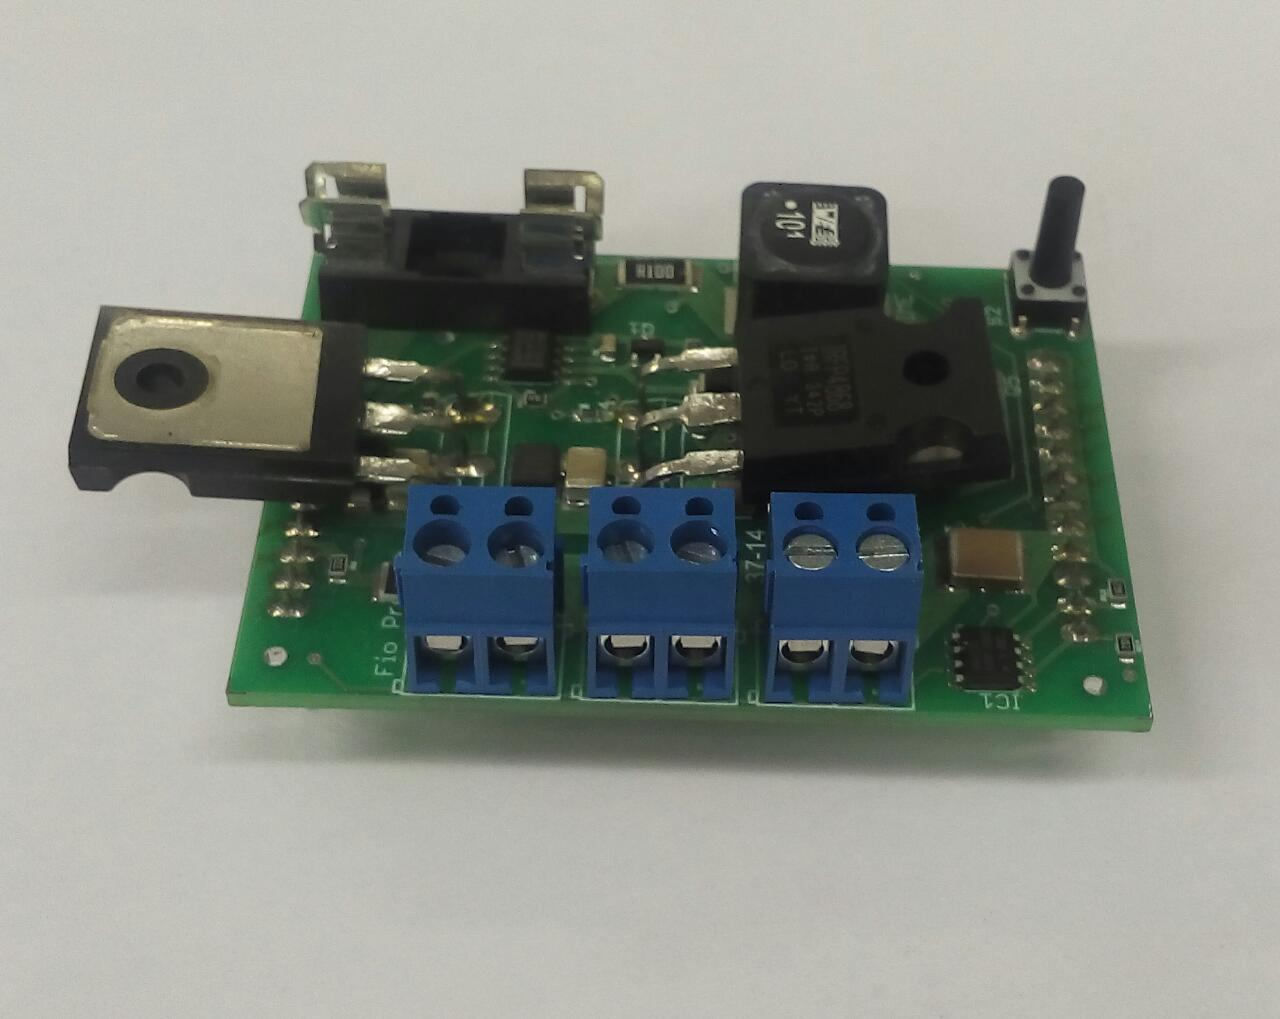
\includegraphics[width=0.8\linewidth]{img/modulochute}
	\caption{Módulo do chute}
	\label{img:modulochute}
\end{figure}

A placa funciona através de um circuito de conversão DC-DC controlado pelo circuito integrado MC34063 que converte os 7,8V DC da bateria em uma saida de 180V DC ligada a dois capacitores eletrolíticos de 2200 $\mu$F e 200V. Além desse circuito existe ainda um circuito para chavear a tensão dos capacitores nos solenoides, o que é feito utilizando um TC4427 \textit{driver} de mosfet e dois mosfets de potência IRFP4868PBF. 

O controle desse módulo é feito através da classe chute que utiliza a classe degrau unitário para limitar a energia transmitida a bola alterando a duração do intervalo de tempo que os mosfets ficarão ativados.

\subsection{Módulo de transmissão}

É o módulo responsável pela comunicação entre a inteligência e o módulo de controle do robô. Consiste em uma placa comercial contendo o \textit{chip} NRF24L01 e os periféricos necessários para o seu uso (ver figura \ref{img:modulotransmissao}).
	
\begin{figure}[thpb]	
    \centering
    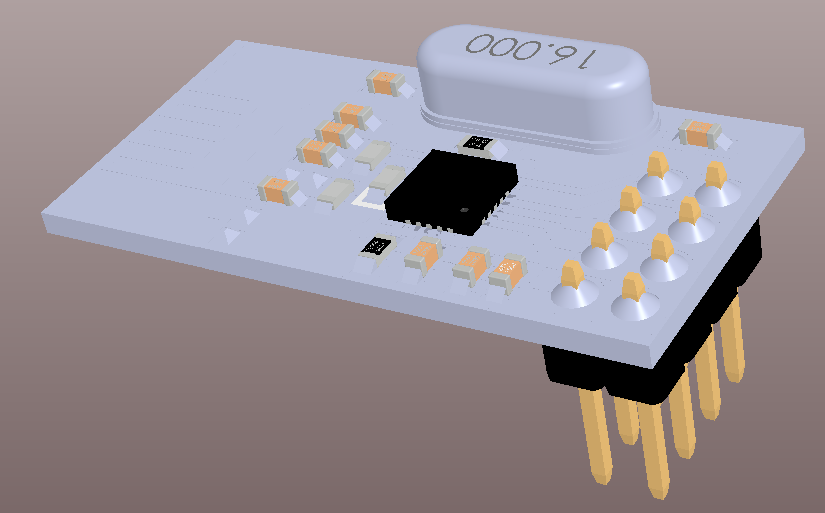
\includegraphics[width=0.9\linewidth]{img/modulotransmissao}
	\caption{Módulo de transmissão. Placa comercial baseada no chip NRF24L01}
	\label{img:modulotransmissao}
\end{figure}
	
O módulo é ligado ao módulo de controle do robô através da placa mãe e se comunica com este utilizando o protocolo SPI (\textit{Serial Peripheral Interface}). Para fazer a comunicação com a inteligência, o módulo se comunica com outro igual ligado ao computador onde a inteligência está sendo executada utilizando uma frequência na faixa de 2,4 GHz.

Para a comunicação entre dois módulos, o \textit{chip} utiliza um protocolo próprio chamado \textit{Enhanced ShockBurst™}, uma camada de vínculo de dados (camada de protocolo que lida com a entrada e saída de sequências de \textit{bits} no meio físico, escondendo das camadas superiores o \textit{hardware} subjacente e lidando com os pacotes perdidos e os pacotes duplicados) que permite envio de pacotes de confirmação sem a necessidade de receptor e transmissor inverterem seus modos de funcionamento (funcionalidade chamada \textit{Auto Acknowledgement}). Isso permite ganhar tempo no envio das informações que a inteligência precisa. 

O \textit{Enhanced ShockBurst™} também permite o uso de até 6 \textit{pipes} para o recebimento de mensagens e o envio de pacotes com tamanho variável. Outras funções desempenhadas são a montagem e desmontagem de pacotes, bem como a validação dos pacotes recebidos, sendo necessário apenas configurar alguns registradores, simplificando o código da transmissão.

Embora o rádio ofereça a opção de usar CRC (\textit{Cyclic Redundancy Check}) para verificar erros nos pacotes, isso não foi usado, pois tornaria a recepção mais lenta (devido à verificação que seria feita) e durante os testes as mensagens nunca chegavam corrompidas.


\section{Design Mecânico}

O robô, figura \ref{fig:robo_3d_e_real}, foi e está sendo desenhado utilizando-se de \textit{software} de CAD (\textit{Computer Aided Design}) e CAM (\textit{Computer Aided Manufacturing}). Várias melhorias e testes estão sendo feitos para melhorar o projeto herdado dos antigos membros da equipe visando principalmente:

a) Deixar o projeto mais simples, se atentando a facilitar a produção das peças e
retirando as desnecessárias;

b) Eficiente, ou seja, que tenhamos uma melhora na precisão do controle e peças
mais resistentes.

A maioria de nossas peças são feitas através de maquinas que utilizam o método CNC(\textit{Computer Numeric Control}) e feitas de alumínio 70-75 apresentando uma alta resistência mecânica e são boas de serem usinadas. Sendo o restante em PLA material utilizado por impressoras 3D e está em estudo para esse ano o uso de peças em plástico injetado em alta pressão.

\begin{figure}[thpb]
    \subfloat{
	    \label{fig:modelado}
        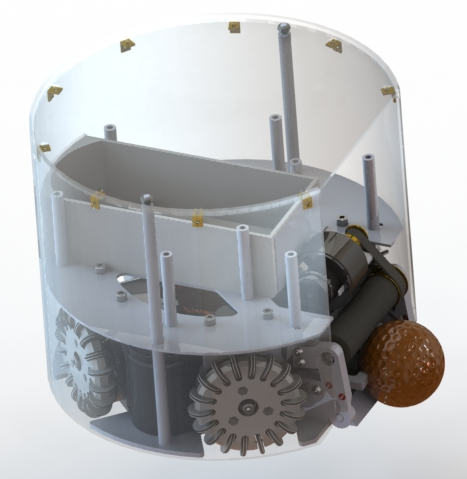
\includegraphics[width=0.47\linewidth]{img/mec1}
    }
    \subfloat{
        \label{fig:real}
        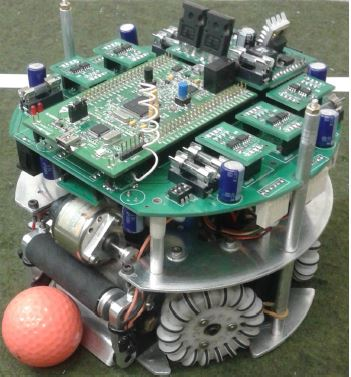
\includegraphics[width=0.47\linewidth]{img/mec2}
    }
    \caption{Vistas do Modelo 3D, \ref{fig:modelado} e robô real, \ref{fig:real}}
    \label{fig:robo_3d_e_real}
\end{figure}

\subsection{Métodos de produção}

\subsubsection {Corte a jato d'água}

Usando corte com jato d’água (\textit{jet-cutting}) produzimos o chassi e a base superior que divide a eletrônica e a bateria do resto do robô, para isso usamos placas de alumínio de 3mm e 2.5 mm, respectivamente, como visto na figura \ref{fig:corte_dagua}.

\begin{figure}[thpb]
    \subfloat{
        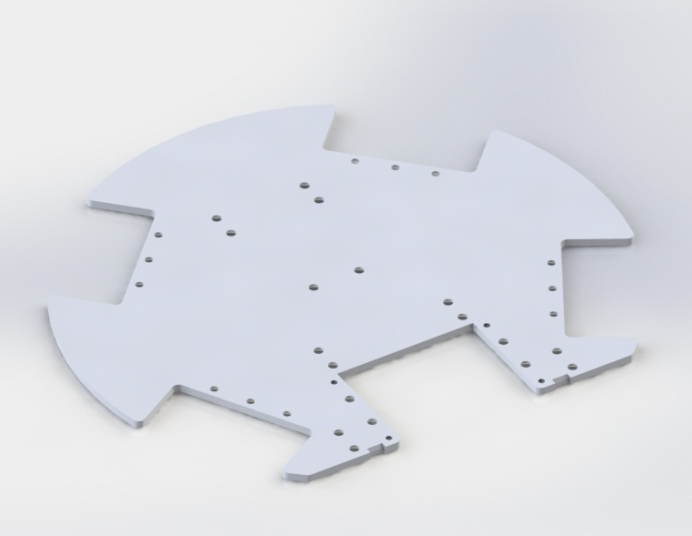
\includegraphics[width=0.47\linewidth]{img/corte_dagua_render}
        \label{img/render3d}
    }
    \subfloat{
        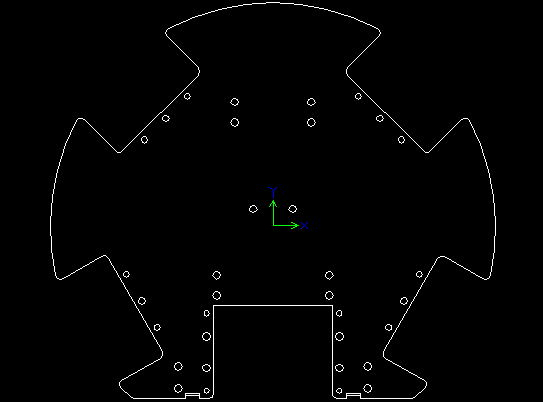
\includegraphics[width=0.47\linewidth]{img/mec4}
        \label{img/fotoreal}
    }
    \caption{Modelo 3D, \ref{img/render3d}, e arquivo DXF, \ref{img/fotoreal}, do chassi do robô.}
    \label{fig:corte_dagua}
\end{figure}


\subsubsection {Fresadora CNC}

Usando a fresadora CNC, produzimos a maioria de nossas peças. Após a modelagem CAD das peças tínhamos que fazer o CAM para gerar o código máquina. Algumas peças foram bastante desafiadoras, tendo em vista o tamanho reduzido e a complexidade de suas formas. Esses dois fatores afetaram principalmente a tirada de referências da peça com o apalpador da máquina, afim de configurar a origem e como prenderíamos essa peça na morsa de maneira segura, principalmente nas últimas fases da produção da peça. Na figura \ref{fig:real_and_model}, um exemplo de peça produzida pela fresadora CNC.

\begin{figure}[thpb]	
	\centering
	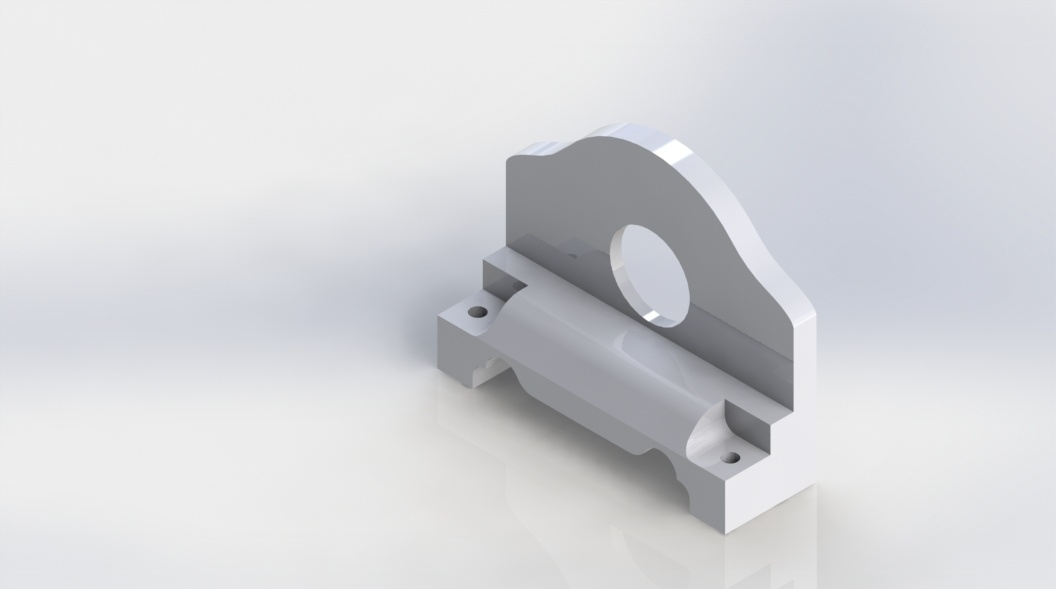
\includegraphics[width=0.9\linewidth]{img/mec6}
	\caption{Modelo 3D de uma das peças do chute}
	\label{fig:real_and_model}
\end{figure}

\subsubsection{Outros}

Por fim foram utilizadas ferramentas como impressora 3D, tornos, jateamento, pneumática seja para produção ou acabamento de peças.


%\subsection{Dimensões}

%Em conformidade com as regras de SSL, a altura do robô é de 149 mm e a projeção máxima do robô no solo é de 180 mm. A altura do driblador é ajustável, de modo que somos capazes de encontrar o ponto ideal para o melhor controle de bola. Utilizando \textit{software} de CAD, fomos capazes de medir a porcentagem de área da bola que estava coberta pelo robô. Obtendo uma porcentagem máxima de cobertura bola de 19,8\%, de acordo com o 20/80 regra da liga.

\subsection{Sistema de transmissão}

Um sistema de engrenagens internas foi feito para transferir a potência dos motores de para as rodas. Esse sistema tem várias vantagens quando comparado com o método tradicional, como evitar a entrada de detritos os motores, cria uma cavidade para aplicar graxa para a lubrificação de engrenagens e um tamanho total menor.

No entanto, existem algumas dificuldades na fabricação dessa peça, principalmente devido ao pequeno tamanho dos dentes, necessários para engrenar com a engrenagem do motor padrão (o motor utilizado é o Hsiang Neng DC escovado motor do tipo HN-GH35GMB). Neste motor a distância entre dois dentes consecutivos é inferior a 1 mm, ficando difícil de usinar a engrenagem interna para essa peça. 

Antigamente foi utilizado impressora 3D para imprimir em plástico ABS a peça, porém as peças não apresentaram bons rendimentos, quebrando a peça e os dentes facilmente, fora que muitas não apresentavam um movimento suave, travando se a força imprimida para sua rotação não fosse significante, o que dificultava o controle do robô, assim estamos estudando realizar o corte das peças utilizando o método de eletroerosão para contornar  problema do pequeno tamanhos dos dentes. Dessa forma seria possível usinar um molde em metal, que serviria para produzir as peças através da técnica de injeção de plástico.

Se essa opção não funcionar, será estudado usinar o molde em impressora 3D, criando uma proteção para a parte em que o molde entra em contato com o bico da injetora. Ou então encomendar o molde de empresa especializada.

\subsection{Chute}

O chute rasteiro, de acordo com a figura  \ref{img:alterarlabel}, é formado por um conjunto de placa de chute, pistão, suporte dianteiro do solenoide, suporte traseiro do solenoide e solenoide. Ele é ativado através de dois capacitores que energizam o solenoide fazendo o pistão, que está aclopado com a placa, ser impulsionado para frente.

Chute alto é formado por placa de chute, suporte único do solenoide, pistão, solenoide, suporte para retenção do pistão. 

Em ambos casos estamos usando ligas para trazer de volta os pistões, por serem baratas e eficientes no processo, porém no caso do chute rasteiro esta sendo estudado o uso de uma mola cônica. Também é possível em ambos casos fazer a volta invertendo a tensão aplicada no solenoide, mas como essa opção consumiria energia da bateria não é tão interessante.

\begin{figure}[thpb]	
	\centering
	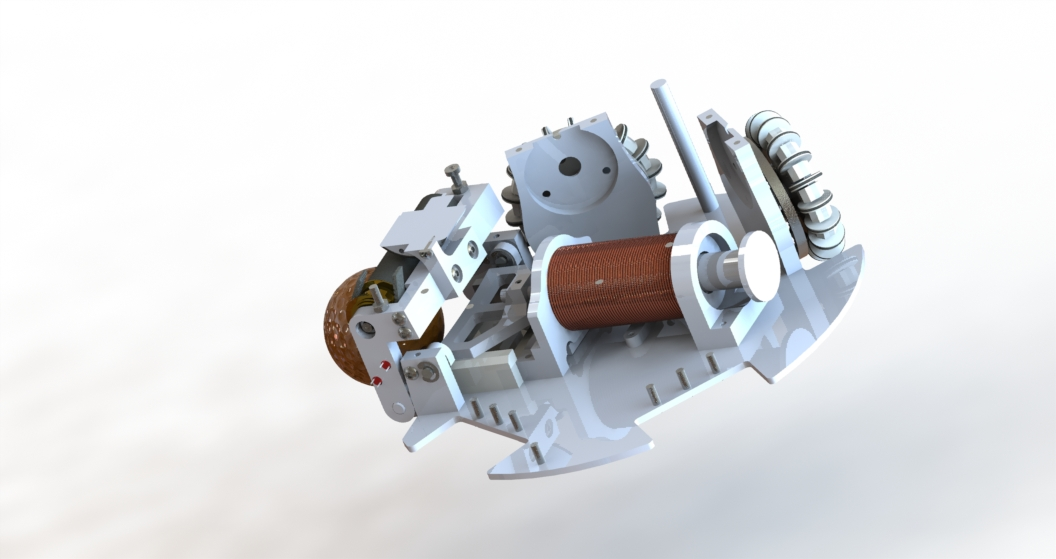
\includegraphics[width=\linewidth]{img/mec11}
	\caption{Imagem renderizada do chute do robô}
	\label{img:alterarlabel}
\end{figure}

\section{Conclusão}

O projeto está sendo reformulado este ano, aumentando o seu caráter modular, para facilitar testes de mudanças estruturais. Isso se traduz no desenvolvimento do Core, que diminui o esforço para o teste de novos algoritmos de inteligência, e na abstração de \textit{hardware} durante a implementação do \textit{firmware} que permite o teste de outros tipos de motor e módulo de controle.

Está sendo realizado também um esforço para melhorar o algoritmo de controle dos robôs de forma a permitir que a inteligência tenha um controle mais refinado da posição dos robôs no campo. E permitir jogadas mais elaboradas com a possibilidade de passes entre os robôs. 

Esse esforço se traduz na implementação do controle de derrapagem das omni rodas, na implementação de um novo filtro de Kalman e reformulação da comunicação entre os robôs e a inteligência de forma a testar o uso de dados dos \textit{encoders} no algoritmo de controle da inteligência.

\subsection*{Trabalhos futuros}

Além destas implementações, será testado ainda o uso de motores \textit{brushless}, mais precisos que os motores de corrente contínua atuais. Porém, como essa mudança modifica grande parte do projeto mecânico e eletrônico dos robôs ela não será implementada para a competição desse ano.

Estão sendo ainda executados testes para escolher o algoritmo de tomada de decisão que será usado durante a competição. O algoritmo usado nas últimas competições baseado em STP está sendo portado para ser compatível com o core, e serão testados outras arquiteturas como multiagente e o uso de algoritmos de aprendizagem.

\section*{Agradecimentos}

Este trabalho teve o apoio financeiro do Departamento de Ciência e Tecnologia do Exército (DCT), Fundação Carlos Chagas Filho de Amparo a Pesquisa do Estado do Rio de Janeiro (FAPERJ), Fundação Ricardo Franco (FRF) e o apoio técnico da Fábrica de Material de Comunicação e Eletrônica (FMCE/IMBEL). A equipe também destaca a assistência dos engenheiros Luis Renault L. Rodrigues, Clara Luz de S. Santos e Jorge L. de Castilho Jr. da FMCE/IMBEL. Agradecimento especial aos membros anteriores da RoboIME, que não só nos aproximaram do projeto, como também dos engenheiros que aspiramos nos tornar. 

%Mandar um salve ai pro apoio financeiro do dct, fundação ricardo franco e faperj e para o apoio da fmce-imbel

%This research was partially supported by Fundacao Carlos Chagas Filho de Amparo a Pesquisa do Estado do Rio de Janeiro -FAPERJ(grant E-26/111.362/2012); Fundacao Ricardo Franco (FRF) and Fabrica de Material de Comunica¸c˜ao e Eletronica (FMCE/IMBEL). The team also acknowledges the assistance of Mr. Carlos Beckhauser from FMCE. Special thanks to Diego Felix de Almeida, Luis Renault L. Rodrigues, Stefano H. Rodrigues, Thiago A. Navarro do Amaral and Victor L. Horta Ferreira, former team members that made this project possible.

\bibliographystyle{unsrt}
\footnotesize\bibliography{ref}		



\end{document}